
\documentclass[12pt]{article}
\usepackage{graphics,amssymb,amsmath}

\usepackage[slovak]{babel}
\usepackage[utf8]{inputenc}
\usepackage[IL2]{fontenc}

\usepackage{multicol}
\usepackage{mathtools}

\pagestyle{empty}
\setlength\textwidth{170mm}
\setlength\textheight{265mm}
\addtolength\oddsidemargin{-20mm}
\addtolength\topmargin{-20mm}
\setlength{\parindent}{1pt}
\setlength{\parskip}{10pt}
\newcount\pocet
\pocet = 1
\def\pr{{\bf \the \pocet .\ \global\advance\pocet by 1}}

\newcommand{\g}{ \dots \dots \dots \dots \dots \ }
\newcommand{\gu}{ \dots \dots \ }
\newcommand{\gr}{\dotfill \ }

\begin{document}

\newenvironment{itemize*}
{\begin{itemize}
\setlength{\itemsep}{0pt}
\setlength{\parskip}{0pt}}
{\end{itemize}}

\newenvironment{enumerate*}
{\begin{enumerate}
\setlength{\itemsep}{0pt}
\setlength{\parskip}{0pt}}
{\end{enumerate}}


\phantom{a}

\centerline{\textbf{\Large Matematika I}}
\smallskip
\centerline{05. január 2020}
\centerline{9:00}
\vskip0.5cm

\centerline{\bf  Meno a priezvisko: \gr Podpis: \gr}
\vskip0.5cm
\centerline{\bf  Ročník: \gr študijný program: \gr}
\vskip0.5cm

\medskip

\pr (11b) Daná je všeobecná rovnica kužeľosečky $9x^2+4y^2-36x-24y-36=0$.\\
\textbf{Doplňte}
\begin{enumerate}
\item[a)] Stredová rovnica kužeľosečky je\gr
\item[b)] Kužeľosečka je \gr typu.
\item[c)] Popíšte (ak existujú):
\begin{enumerate}
\item[$c_1$)] dĺžka hlavnej poloosi je \gr
\item[$c_2$)] dĺžka vedľajšej poloosi je \gr
\item[$c_3$)] excentricita je \gr
\end{enumerate}
\item[d)] Napíšte súradnice (ak existujú):
\begin{itemize}
\item[$d_1$)] hlavných vrcholov kužeľosečky \gr
\item[$d_2$)] vedľajších vrcholov kužeľosečky \gr
\item[$d_3$)] súradnice ohniska resp. ohnísk kužeľosečky \gr
\end{itemize}
\item[e)] Znázornite kužeľosečku a v náčrte popíšte jej významné prvky.
\end{enumerate}


\newpage

\pr (2b) Vyberte funkciu, ktorej definičný obor je znázornený na nasledujúcom obrázku.

\begin{multicols}{2}
\scalebox{0.65}{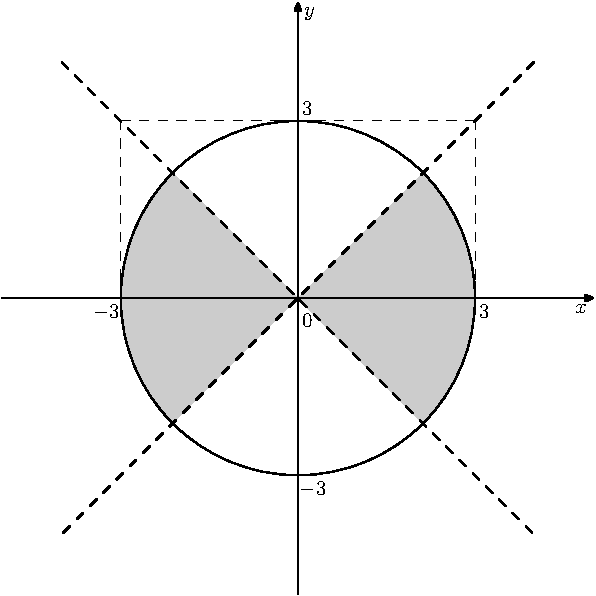
\includegraphics{Df.pdf}}

\begin{itemize}
\item[a)] $\displaystyle f(x,y)= \ln{(9-x^2-y^2)}+\ln{(x^2-y^2)}$
\item[b)] $\displaystyle f(x,y)= \sqrt{9-x^2-y^2}+\ln{(x^2-y^2)}$
\item[c)] $\displaystyle f(x,y)= \sqrt{9-x^2-y^2}+\ln{(x^2+y^2)}$
\item[d)] $\displaystyle f(x,y)= \sqrt{9-x^2-y^2}+\sqrt{x^2-y^2}$
\end{itemize}
\end{multicols}

Test prikladu 3

\end{document}